% ============ §5 模型的建立与求解 ============
\section{模型的建立与求解}

\subsection{问题一：常热物性瞬态传热与非线性水分扩散模型}

\subsubsection{烘房环境辨识与平台外推}

附件 1 给出 0--4 h 烘房温度与水分浓度的采样（60 s 间隔），数据呈单调
爬升至平台的一阶惯性环节形态（加热/加湿系统的标准动态特性），因此辨识为

\begin{equation}
T_{env}(t)=T_\infty-(T_\infty-T_0)\,e^{-t/\tau}
\end{equation}

最小二乘拟合得 $\tau=1776$ s、$R^2=0.9973$（水分浓度同理，$\tau=2522$ s、
$R^2=0.9944$）；拟合残差用保形三次样条光滑后叠加，使模型在数据点处与附件 1
一致（图~\ref{fig:env}）。$t\ge7200$ s 平台期统计为 $49.97\pm0.17$\,°C 与
$0.0500\pm0.0002$ kg/kg，噪声与均值之比小于 0.4\%，据此将 $t>4$ h 的
边界条件外推为恒值（问题二使用）。环境辨识的另一个用途是：指数边界下
温度场存在闭式解析解，可作为数值求解器的独立基准。

\begin{figure}[H]
\centering
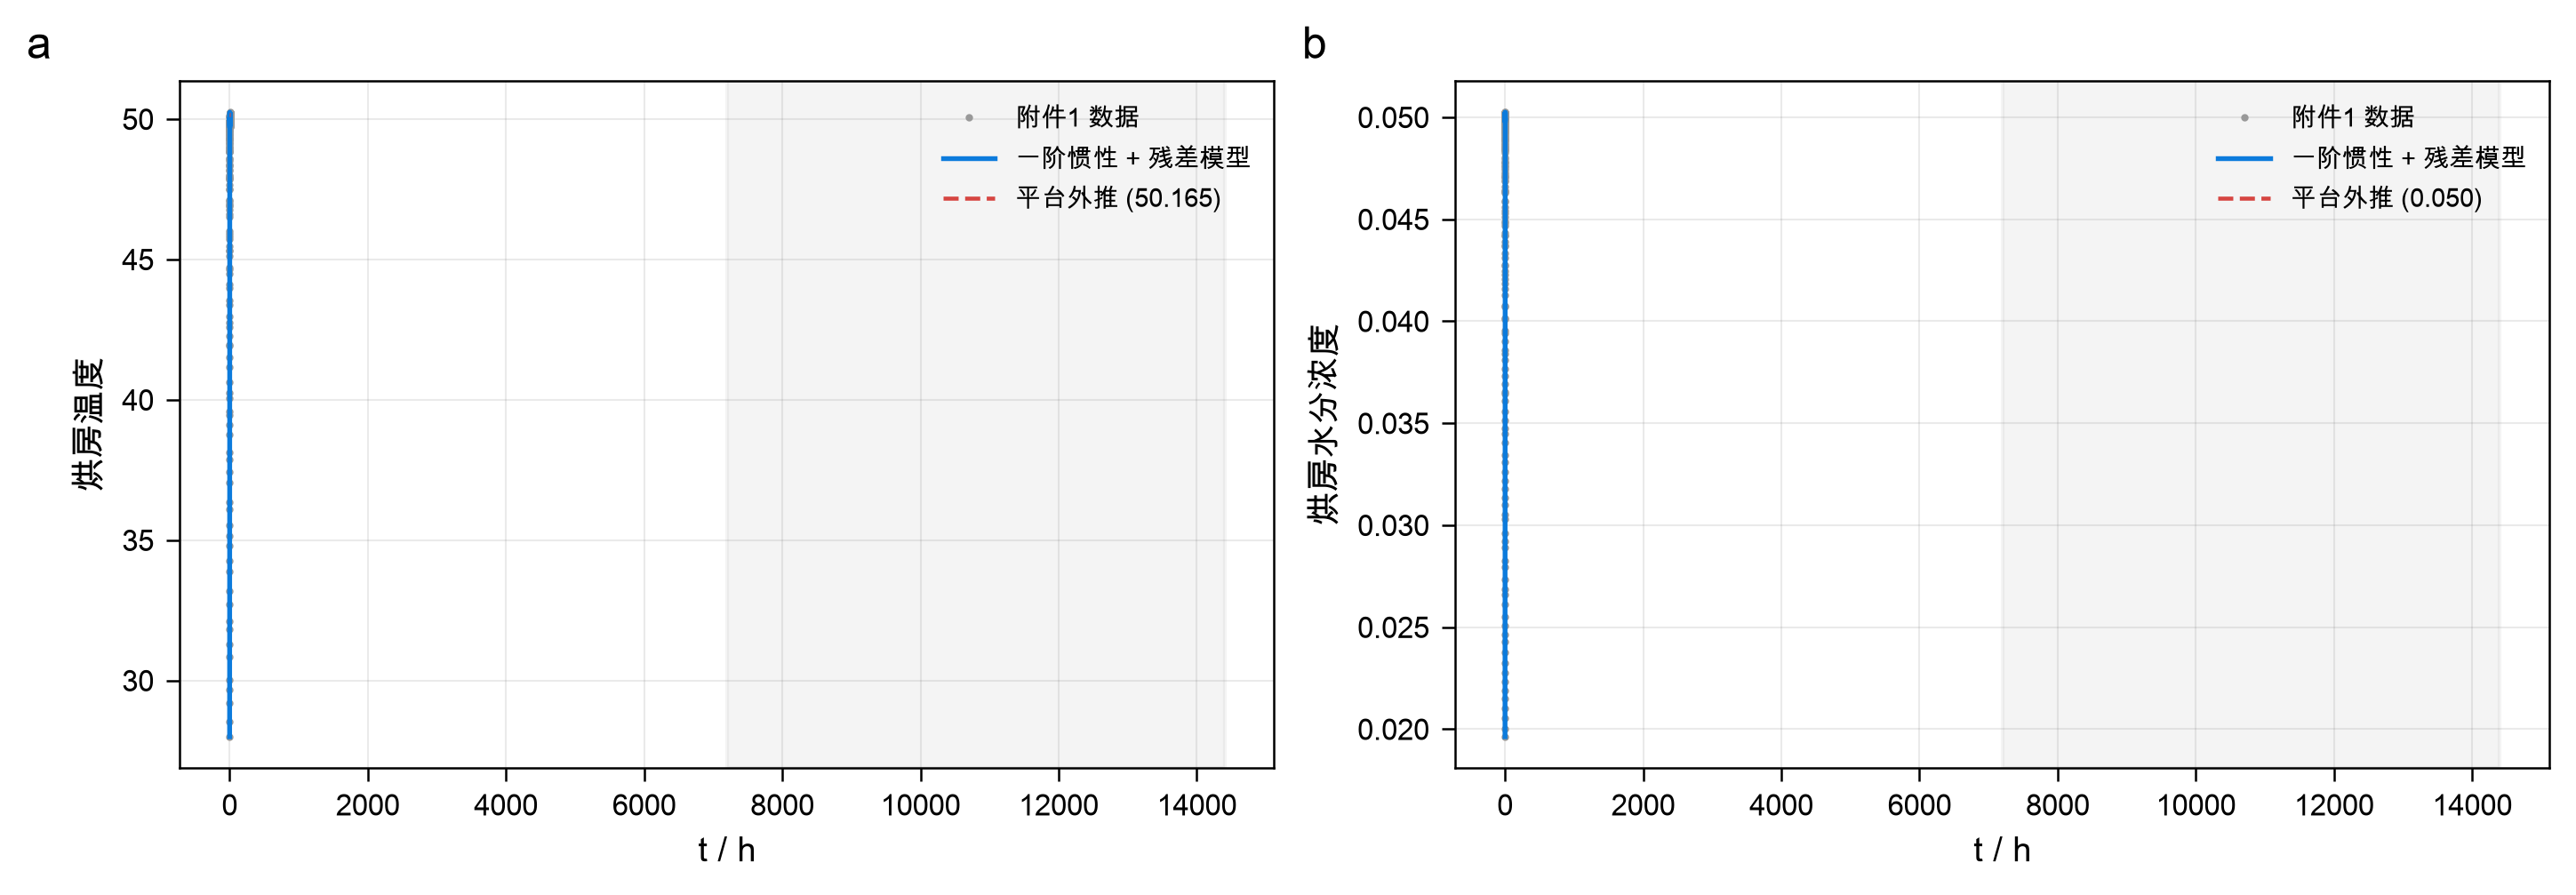
\includegraphics[width=0.95\textwidth]{fig6_env_model.png}
\caption{烘房环境的一阶惯性辨识。数据点、辨识模型与平台期统计区间（阴影）。
左：温度（$R^2=0.9973$，$\tau=1776$ s）；右：水分浓度（$R^2=0.9944$，
$\tau=2522$ s）。}
\label{fig:env}
\end{figure}

\subsubsection{温度场解析解}

预热阶段温度场满足常物性轴对称热传导方程

\begin{equation}
\rho c_p\frac{\partial T}{\partial t}=\frac{k}{r}\frac{\partial}{\partial r}\left(r\frac{\partial T}{\partial r}\right)
\end{equation}
\begin{equation}
T(r,0)=T_0,\qquad \left.\frac{\partial T}{\partial r}\right|_{r=0}=0,\qquad
-\left.k\frac{\partial T}{\partial r}\right|_{r=R}=h\big(T(R,t)-T_{env}(t)\big)
\end{equation}

（$\rho=820$ kg/m$^3$、$c_p=2600$ J/(kg·K)、$k=0.36$ W/(m·K)、
$h=25$ W/(m$^2$·K)，附录 2）。对流边界的特征值问题为
$\lambda J_1(\lambda)=\mathrm{Bi}\,J_0(\lambda)$，$\mathrm{Bi}=hR/k=1.39$。
对该特征展开应用 Duhamel 原理（推导过程见附录 A），指数边界主项可显式求积，
残差经递归卷积修正，最终

\begin{equation}
T(r,t)=T_{fit}(t)-\Delta T\sum_{n=1}^{80}A_n J_0\!\left(\frac{\lambda_n r}{R}\right)g_n(t)
+\delta(t)-\sum_{n=1}^{80}A_n J_0\!\left(\frac{\lambda_n r}{R}\right)I_n(t)
\end{equation}

其中 $T_{fit}(t)=T_\infty-\Delta T\,e^{-t/\tau}$ 为辨识主项，$\delta(t)$ 为
环境残差，$g_n$、$I_n$ 与系数 $A_n$ 的定义见附录 A。该式对任意输出时刻
无需时间步进，级数截断误差在 $10^{-9}$ 量级，满足 4 位小数要求；$\tau\to0$
时退化为阶跃边界响应，与 Bessel 级数解逐点一致到 $5\times10^{-9}$。
这一解析解同时作为谱配点求解器的独立基准（图~\ref{fig:duhamel}）。

\begin{figure}[H]
\centering
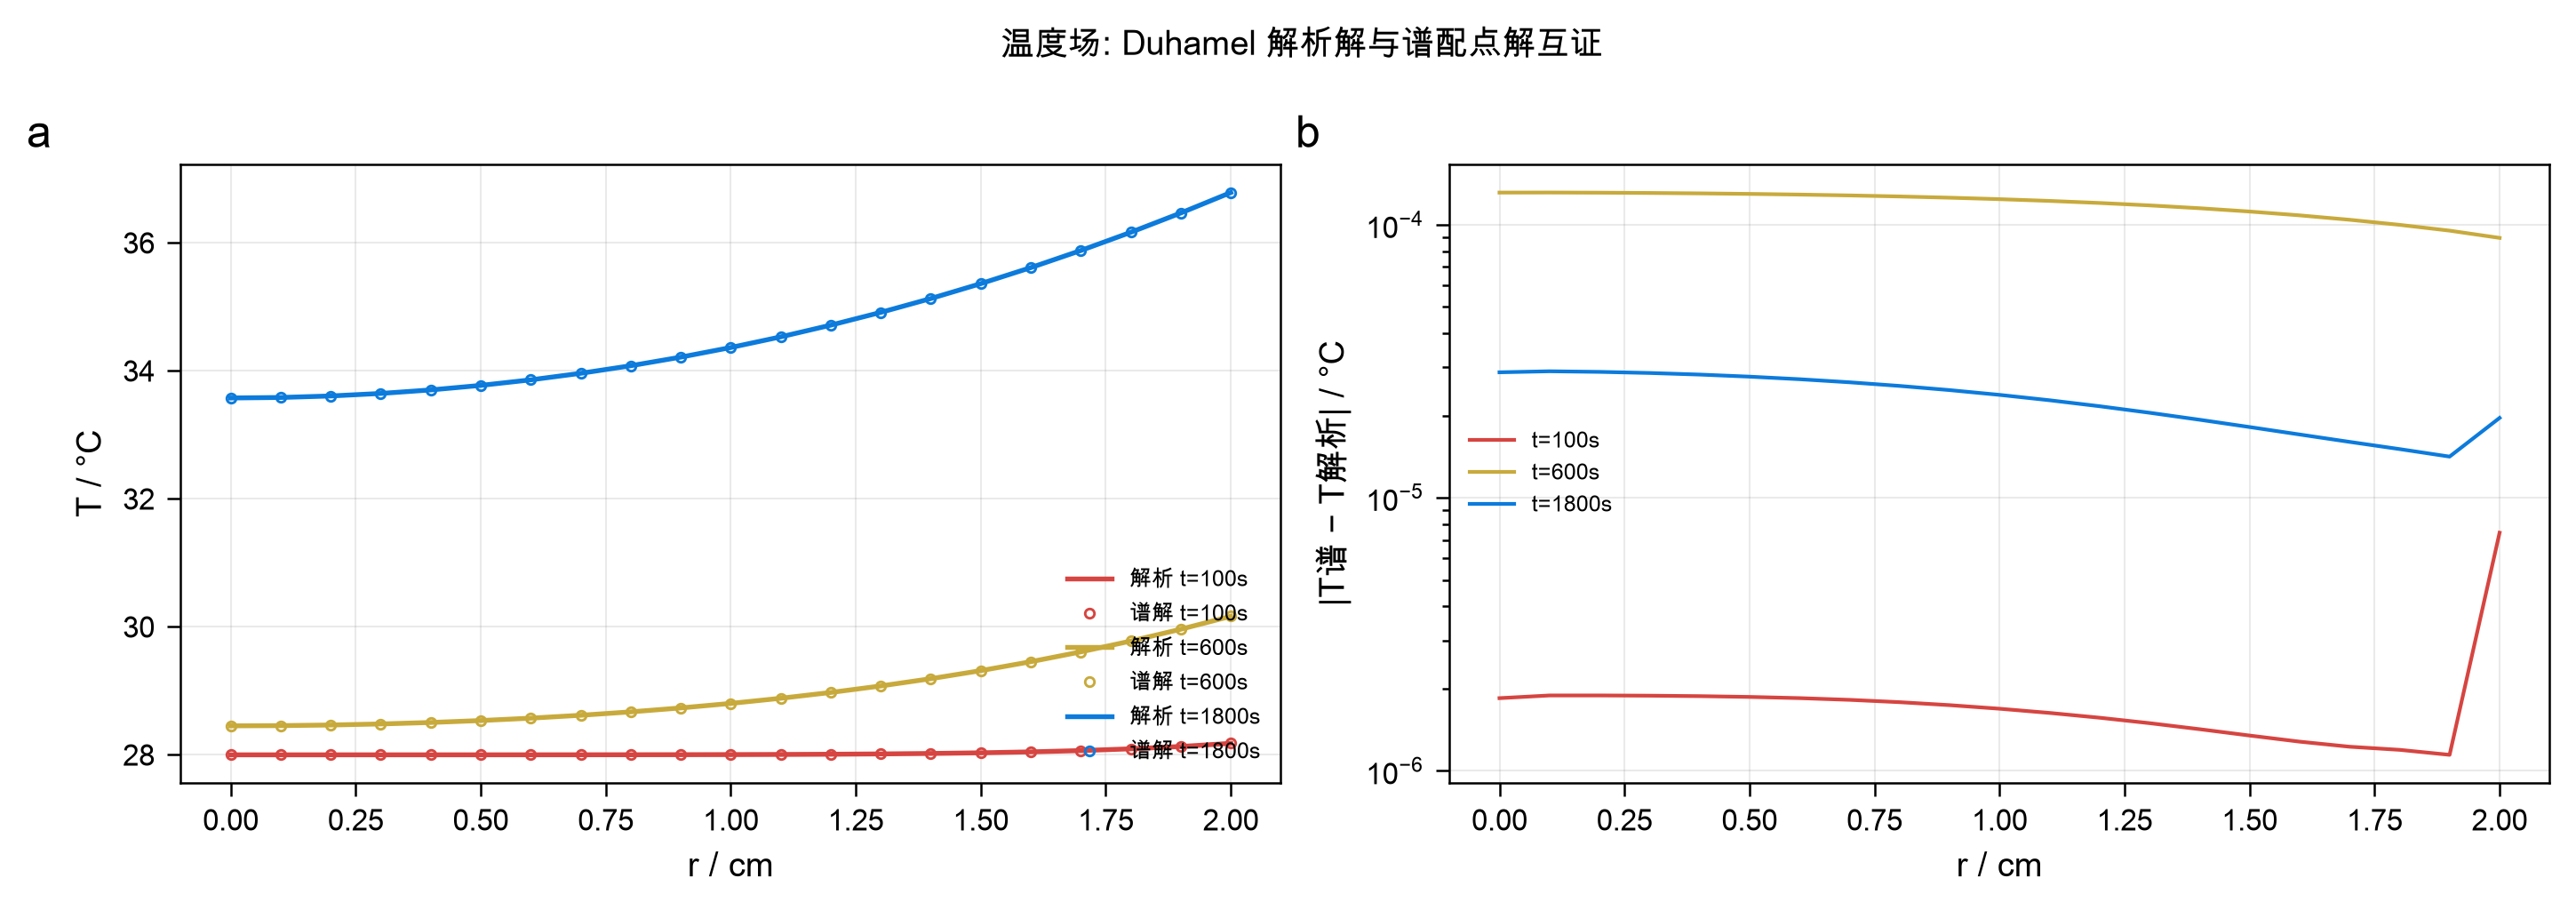
\includegraphics[width=0.95\textwidth]{fig2_duhamel.png}
\caption{温度场解析解与谱配点解的对比（a）及逐点偏差（b）。最大偏差
$1.6\times10^{-4}$\,°C，两种求解方式相互印证。}
\label{fig:duhamel}
\end{figure}

\subsubsection{水分场与统一数值离散}

水分场满足非线性扩散方程

\begin{equation}
\frac{\partial C}{\partial t}=\frac{1}{r}\frac{\partial}{\partial r}\left(r\,D(C)\frac{\partial C}{\partial r}\right),\qquad
D(C)=7\times10^{-9}e^{-0.89/C}
\end{equation}

初值 $C(r,0)=2.55$，表面条件 $-D\,\partial C/\partial r=\beta(C-C_{env})$，
$\beta=8\times10^{-7}$ m/s。温度方程与水分方程没有直接的双向作用（热物性
为常数，$D$ 不含温度），水分方程经 $D(C)$ 单向依赖于自身场。

空间离散采用 Chebyshev--Gauss--Lobatto 谱配点（$N$ 个模式，$r=R(1-x)/2$
映射），一阶微分矩阵按 Trefethen 公式给出\cite{trefethen}；扩散项按乘积
链式离散，即对 $rD(C)\,C_r$ 整体微分，该形式在轴心处保持正则（展开形式
$C_{rr}+C_r/r$ 在轴心附近的谱离散不稳定，具体分析见附录 B）。轴心与表面
两个边界节点不作为时间积分状态，而在每次右端求值中由对称条件与 Robin
条件解出（边界方程求解与选支处理的细节见附录 B）。半离散系统用自适应
隐式 BDF 积分，末位 Chebyshev 系数作为后验误差指示\cite{gasparin}：
问题一解在 $t=1800$ s 时末位系数 $5.1\times10^{-13}$（图~\ref{fig:spectral}），
远低于 4 位小数阈值。该离散框架为问题二至四的统一求解内核。

\begin{figure}[H]
\centering
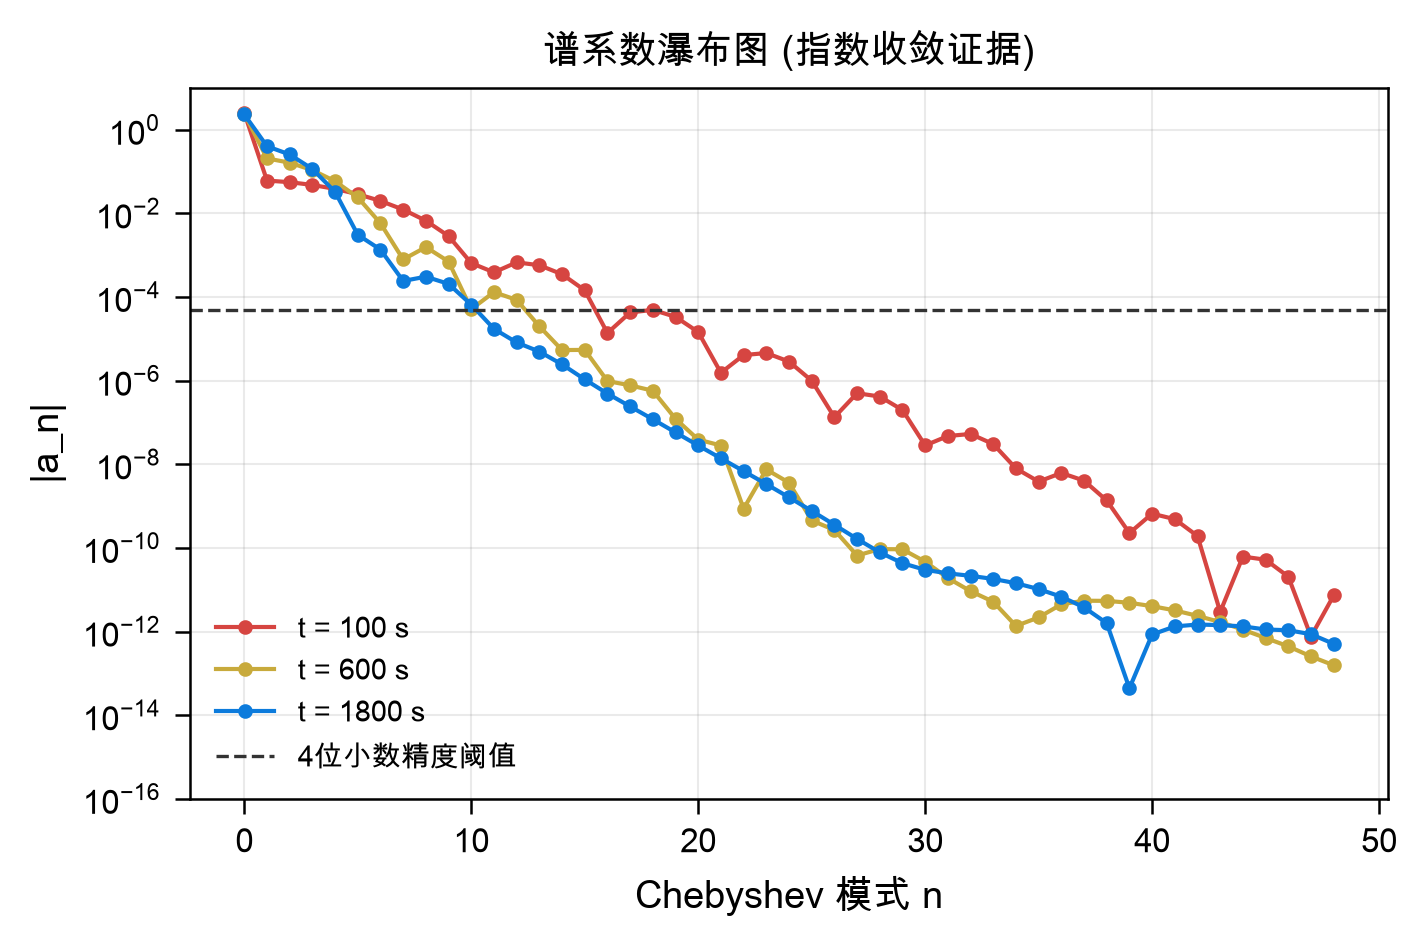
\includegraphics[width=0.62\textwidth]{fig1_spectral.png}
\caption{谱系数随模式数指数衰减（$t=1800$ s）。末位系数 $5\times10^{-13}$
远低于 4 位小数精度阈值 $5\times10^{-5}$。}
\label{fig:spectral}
\end{figure}

\subsubsection{结果}

表~\ref{tab:q1t}、\ref{tab:q1c}（分别按题目表 1、表 2 格式输出，完整数据
见 result1.xlsx）：30 min 内表面温度由 28.00\,°C 升至 36.79\,°C
（100 s 时 28.18\,°C），中心升至 33.58\,°C；表面含水率由 2.5500 降至
1.5102 kg/kg，中心保持 2.5500 kg/kg。图~\ref{fig:preheat} 以二维热图
与径向剖面给出时空演化：温度场整体爬升并形成径向梯度，水分仅在表面薄层
下降。这与无量纲估计一致（$\mathrm{Fo}_T=0.76$、$\mathrm{Fo}_m=0.022$）：
预热阶段工艺目标是快速均温、尽量保持内部水分。

\begin{figure}[H]
\centering
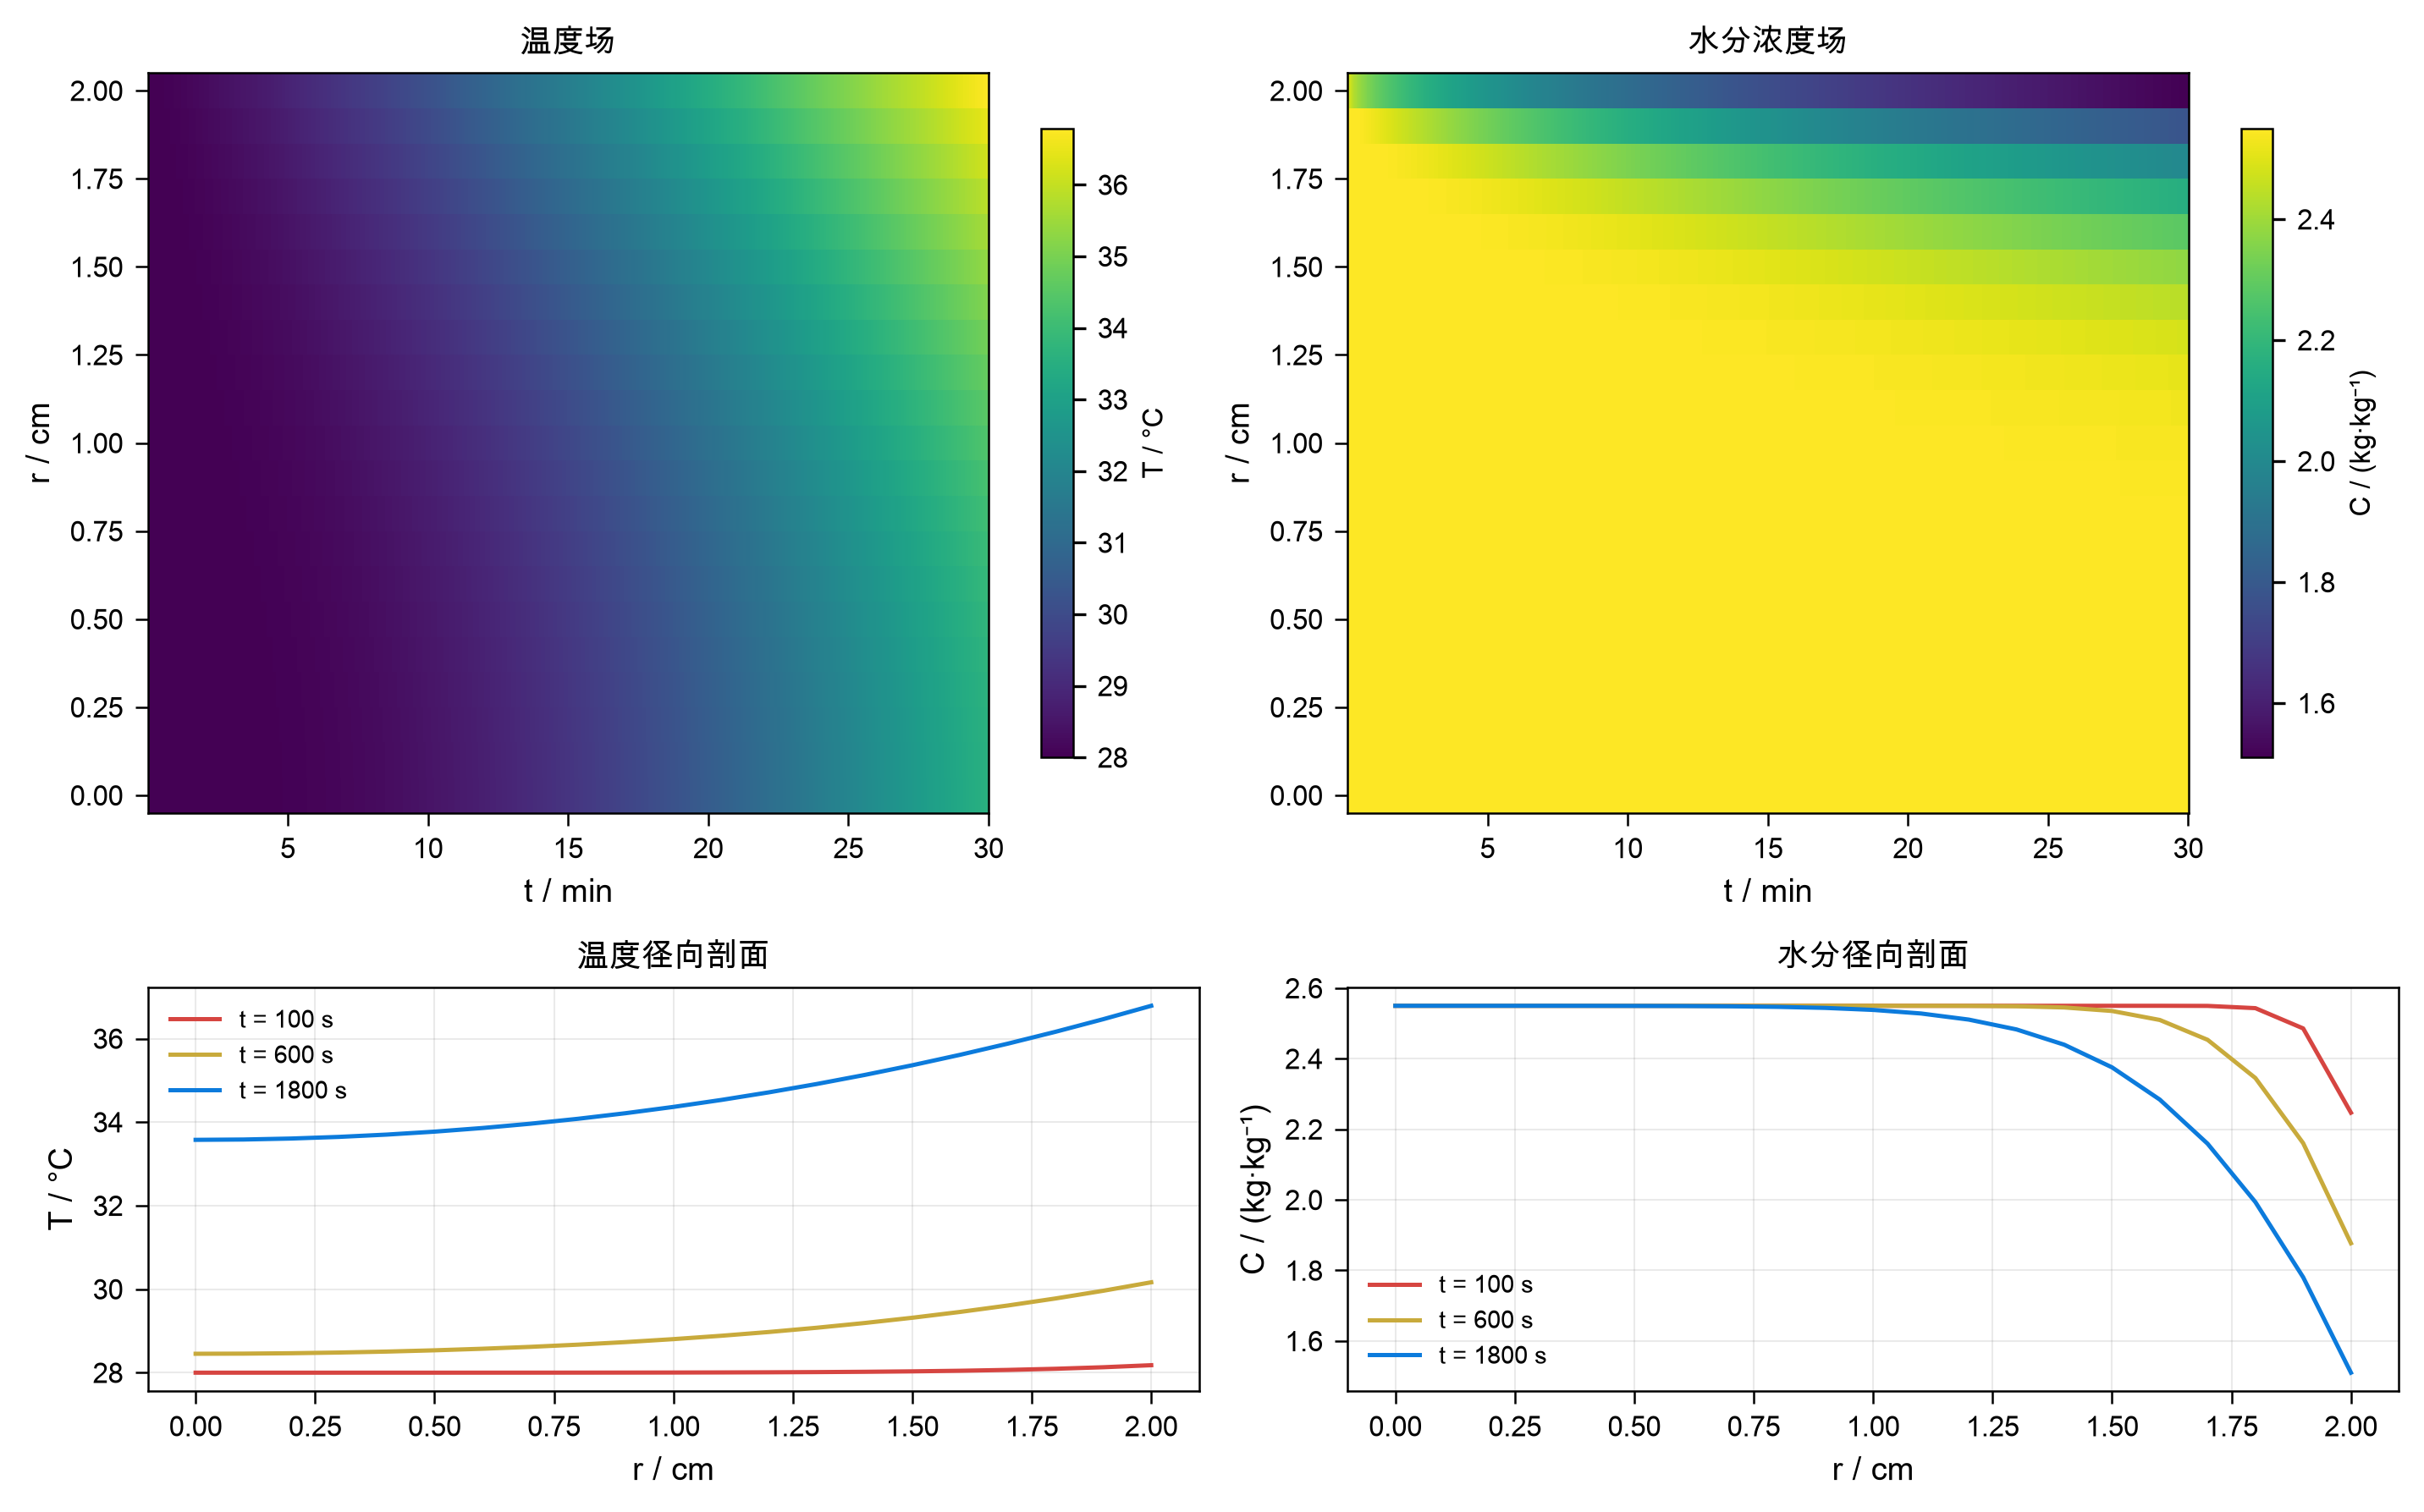
\includegraphics[width=0.95\textwidth]{fig3_preheat.png}
\caption{预热阶段时空演化（二维热图，上）与典型时刻径向剖面（下）。
左列温度，右列水分浓度。}
\label{fig:preheat}
\end{figure}

\begin{table}[H]
\centering
\caption{30 分钟内药材的温度（按题目表 1 的格式要求输出，完整数据见 result1.xlsx）}
\label{tab:q1t}
\begin{tabular}{c|ccccc}
\toprule
时间/s & 0 cm & 0.5 cm & 1 cm & 1.5 cm & 2 cm \\
\midrule
100 & 28.0000 & 28.0003 & 28.0038 & 28.0317 & 28.1792 \\
300 & 28.0405 & 28.0632 & 28.1509 & 28.3668 & 28.8483 \\
600 & 28.4530 & 28.5357 & 28.8035 & 29.3156 & 30.1646 \\
900 & 29.3240 & 29.4581 & 29.8756 & 30.6164 & 31.7295 \\
1200 & 30.5428 & 30.7099 & 31.2225 & 32.1128 & 33.4284 \\
1500 & 31.9960 & 32.1871 & 32.7665 & 33.7471 & 35.1196 \\
1800 & 33.5758 & 33.7723 & 34.3644 & 35.3624 & 36.7859 \\
\bottomrule
\end{tabular}
\end{table}

\begin{table}[H]
\centering
\caption{30 分钟内药材的水分浓度（按题目表 2 的格式要求输出，单位 kg/kg）}
\label{tab:q1c}
\begin{tabular}{c|ccccc}
\toprule
时间/s & 0 cm & 0.5 cm & 1 cm & 1.5 cm & 2 cm \\
\midrule
100 & 2.5500 & 2.5500 & 2.5500 & 2.5500 & 2.2470 \\
300 & 2.5500 & 2.5500 & 2.5500 & 2.5492 & 2.0508 \\
600 & 2.5500 & 2.5500 & 2.5500 & 2.5353 & 1.8770 \\
900 & 2.5500 & 2.5500 & 2.5497 & 2.5045 & 1.7547 \\
1200 & 2.5500 & 2.5500 & 2.5482 & 2.4646 & 1.6586 \\
1500 & 2.5500 & 2.5499 & 2.5445 & 2.4206 & 1.5787 \\
1800 & 2.5500 & 2.5497 & 2.5383 & 2.3755 & 1.5102 \\
\bottomrule
\end{tabular}
\end{table}


\subsubsection{验证}

\begin{enumerate}
\item 解析基准：谱配点温度解与 5.1.2 解析解逐点对比，最大偏差
$1.6\times10^{-4}$\,°C（图~\ref{fig:duhamel}）；
\item 常扩散系数情形的谱解与 Bessel 级数解偏差 $9.5\times10^{-9}$；
\item 独立算法交叉验证：与有限体积法求解器（400 节点，网格收敛验证后）
对比，表~\ref{tab:q1t}、\ref{tab:q1c} 逐项 4 位小数一致。
\end{enumerate}
